Per valutare il comportamento della rete si sono utilizzate 100 mappe quadrate 
di lato 10 e di lato 5. Il numero di lattine selezionato è stato scelto in 
maniera proporzionale fra le mappe ed è quindi 50 per le mappe di lato 10 e 13 
per le mappe di lato 5. Gli altri parametri sono stati scelti tramite varie 
esecuzioni di prova per valutarne l'impatto sulla performance. Il numero di 
passi che i Robby possono effettuare è stato selezionato per impedire la 
strategia banale che attraversa l'intera mappa per esplorarla e raccogliere le 
lattine. Da test che non verranno qua analizzati in dettaglio è emerso che con 
un numero sufficiente di round il sistema è in grado di raccogliere fino al 
99\% delle lattine.
\\
Nei test da noi effettuati, contrariamente a quanto atteso, l'utilizzo della 
vista globale non conduce significativi miglioramenti nelle performance del 
sistema. La ragione di tale inefficienza è probabilmente da ricondurre alla 
incapacità della rete di apprendere il significato del valore contenuto 
nelle celle della known map, che assumono valori variabili nel tempo. Le celle 
lontane dal Robby sono infatti sconosciute finché non vengono osservate e tale 
comportamento non permette un apprendimento efficace.
\\
Riportiamo in seguito una visualizzazione grafica del comportamento del 
programma durante 4000 generazioni, su mappe di dimensione 10:
\begin{figure}[H]
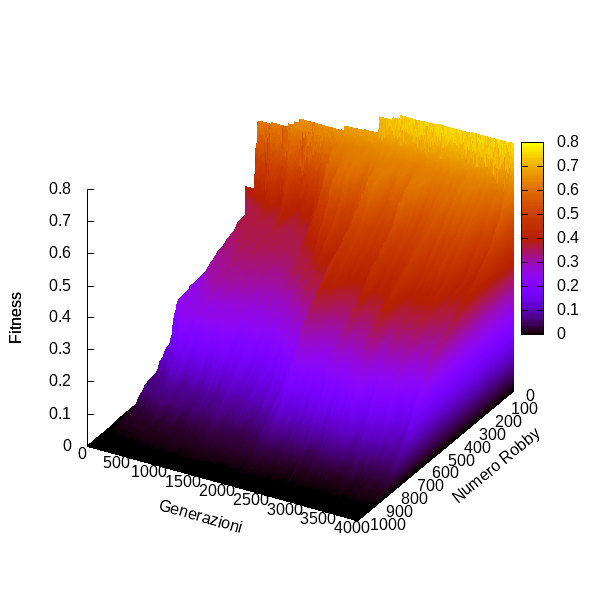
\includegraphics[width=.8\textwidth]{img/graph10x10.png}
\caption{}
\end{figure}
